\begin{figure}[H]
    \centering
    \begin{minipage}[c][9.5cm][c]{0.38\textwidth}
        \centering
        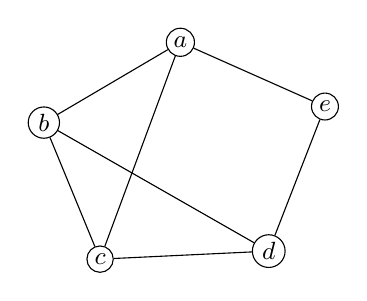
\begin{tikzpicture}[scale=1.02,every node/.style={circle,draw,inner sep=1.4pt,font=\small}]
            \node (a) at (0.0,1.4) {$a$};
            \node (b) at (-1.7,0.4) {$b$};
            \node (c) at (-1.0,-1.3) {$c$};
            \node (d) at (1.1,-1.2) {$d$};
            \node (e) at (1.8,0.6) {$e$};

            \draw (a) -- (b);
            \draw (a) -- (c);
            \draw (a) -- (e);
            \draw (b) -- (c);
            \draw (b) -- (d);
            \draw (c) -- (d);
            \draw (d) -- (e);
        \end{tikzpicture}
        \\\smallskip
        {\small Input graph $G$.}
        \\\medskip
        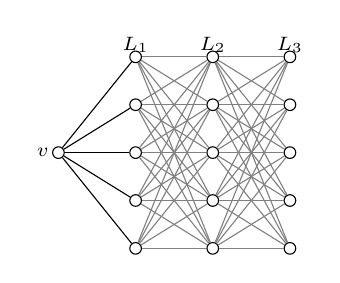
\begin{tikzpicture}[
            x=0.98cm,
            y=0.76cm,
            vertex/.style={circle,draw,inner sep=0pt,minimum size=4.2pt},
            note/.style={draw=none,font=\scriptsize}
        ]
            \node[vertex] (v) at (0,0) {};
            \node[note,left] at (v) {$v$};

            \node[note] at (1,1.8) {$L_1$};
            \node[note] at (2,1.8) {$L_2$};
            \node[note] at (3,1.8) {$L_3$};

            \foreach \i/\y in {1/1.6,2/0.8,3/0,4/-0.8,5/-1.6} {
                \node[vertex] (a\i) at (1,\y) {};
                \node[vertex] (b\i) at (2,\y) {};
                \node[vertex] (c\i) at (3,\y) {};
            }

            \foreach \i in {1,...,5} {
                \draw (v) -- (a\i);
            }
            \foreach \i in {1,...,5} {
                \foreach \j in {1,...,5} {
                    \draw[gray] (a\i) -- (b\j);
                    \draw[gray] (b\i) -- (c\j);
                }
            }
        \end{tikzpicture}
        \\\smallskip
        {\small A single gadget $H^v$ for $n(G)=5$ and $d=3$.}
    \end{minipage}
    \hfill
    \begin{minipage}[c][9.5cm][c]{0.58\textwidth}
        \centering
        \begin{tikzpicture}[
            x=1.05cm,
            y=1.05cm,
            scale=1.12,
            transform shape,
            vertex/.style={circle,draw,fill=white,inner sep=1.2pt,font=\scriptsize},
            gadget/.style={circle,draw,inner sep=0pt,minimum size=2.1pt,draw=cutC,fill=cutC!30},
            gadgetedge/.style={draw=cutC!75,line width=0.22pt}
        ]
            \coordinate (a) at (0.0,1.1);
            \coordinate (b) at (-1.3,0.4);
            \coordinate (c) at (-0.9,-0.95);
            \coordinate (d) at (0.7,-0.9);
            \coordinate (e) at (1.4,0.5);

            \draw (a) -- (b);
            \draw (a) -- (c);
            \draw (a) -- (e);
            \draw (b) -- (c);
            \draw (b) -- (d);
            \draw (c) -- (d);
            \draw (d) -- (e);

            \foreach \name/\ang in {a/90,b/165,c/240,d/312,e/18} {
                \begin{scope}[shift={(\name)}, rotate=\ang]
                    \foreach \i/\yy in {1/0.52,2/0.26,3/0,4/-0.26,5/-0.52} {
                        \node[gadget] (\name1\i) at (0.78,\yy) {};
                        \node[gadget] (\name2\i) at (1.44,\yy) {};
                        \node[gadget] (\name3\i) at (2.1,\yy) {};
                    }
                    \foreach \i in {1,...,5} {
                        \draw[gadgetedge] (0,0) -- (\name1\i);
                    }
                    \foreach \i in {1,...,5} {
                        \foreach \j in {1,...,5} {
                            \draw[gadgetedge] (\name1\i) -- (\name2\j);
                            \draw[gadgetedge] (\name2\i) -- (\name3\j);
                        }
                    }
                \end{scope}
            }

            \node[vertex] at (a) {$a$};
            \node[vertex] at (b) {$b$};
            \node[vertex] at (c) {$c$};
            \node[vertex] at (d) {$d$};
            \node[vertex] at (e) {$e$};
        \end{tikzpicture}
        \\\smallskip
        {\small The graph $H$.}
    \end{minipage}
    \caption{Reduction from Theorem~\ref{thm:hac-d-inapproximability} for $n(G)=5$ and $d=3$. The left side shows the input graph and a single gadget $H^v$, while the right side shows the full graph $H$.}
    \label{fig:hardness-diameter-reduction}
\end{figure}